
The efficiency and acceptance of the neutron detection system varies greatly over its opening angle range of 20$^{\circ}$ to 180$^{\circ}$, as illustrated in Fig.~\ref{fig:DetAcceptance}.
This is both due to the neutron detection system's non-spherical symmetry and to varying efficiency as a function of particle position on the detector.
In order to give a result that is sensitive to angular correlations, but is highly insensitive to detector efficiencies and experimental drifts in PMT voltage, accelerator current, \emph{etc}., the angular correlation is determined by dividing a correlated neutron distribution by an uncorrelated neutron distribution. That is,
\begin{equation}
\label{eq:angularCorr}
\text{angular correlation }  = \frac{nn_{\text{corr}}(\theta)}{nn_{\text{uncorr}}(\theta)},
\end{equation}
where $nn_{\text{corr}}(\theta)$ is the n-n yield after the subtraction of accidental n-n coincidences, and $nn_{\text{uncorr}}(\theta)$ is a contrived distribution of uncorrelated n-n pairs, which is produced by pairing neutron events that occurred during different pulses.
%\footnote{A neutron event is the detection of a particle with a ToF between of 35 and 130 ns (see Fig.~\ref{fig:ToF}b). All n-n yields are normalized per accelerator pulse.}
The subtraction of accidental n-n coincidences to produce $nn_{\text{corr}}(\theta)$ amounts to a 10\% correction, the procedure of which is covered in section~\ref{Reconstruction of Accidental Coincidence}. The construction of $nn_{\text{uncorr}}(\theta)$ is described in detail in section~\ref{subsec:SPDPCancelation}.

\subsection{Cancelation of Detector Efficiencies, Drifts, and Geometric Phase Space}
\label{subsec:SPDPCancelation}
%\footnote{While this notation implies that coincident events are due solely to neutrons, about 3\% of total  $nn_{\text{corr}}(\theta)$ events are not due to neutrons. This percentage was determined by comparing data from a non-neutron producing Al target to that from a $^{238}$U target (see Fig.~\ref{fig:Noise})} 
\begin{figure}[h]
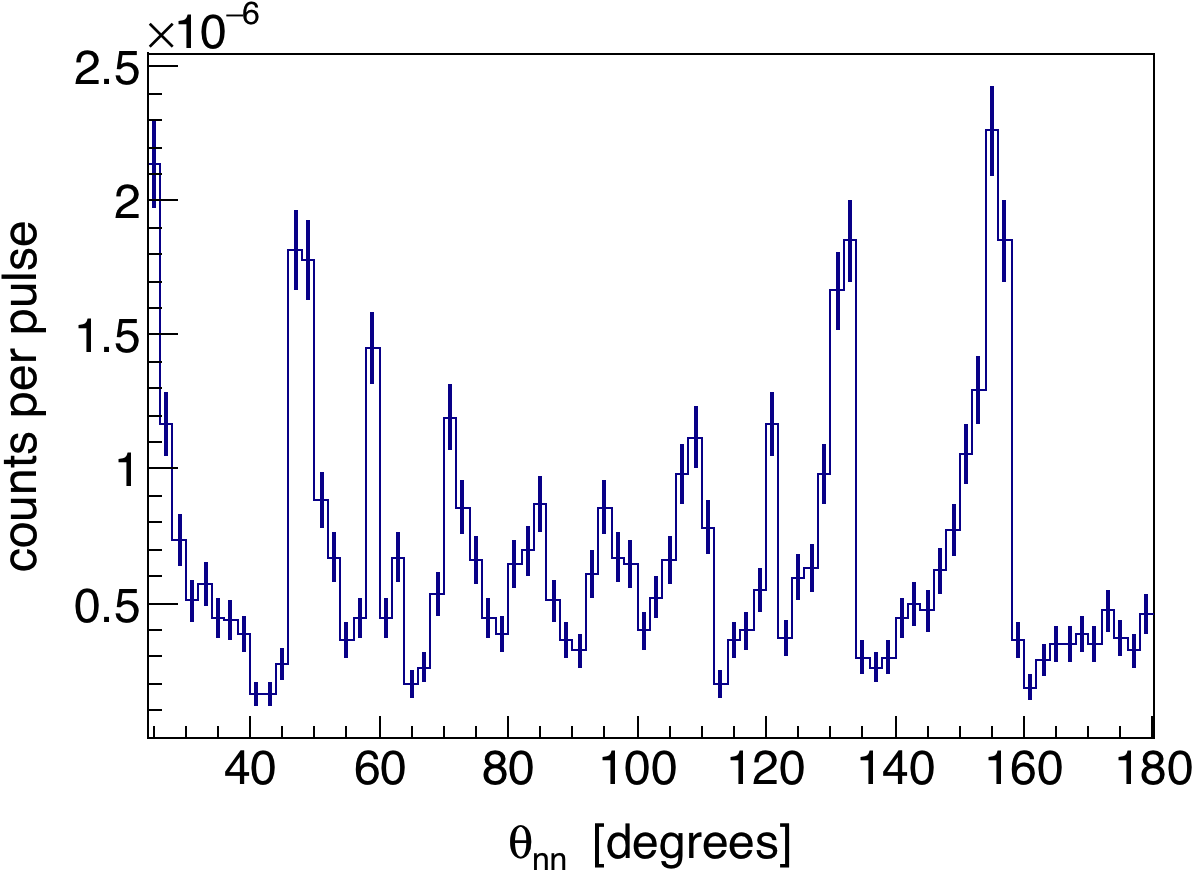
\includegraphics[width=\figsize\textwidth]{./DetAcceptance.png}
\caption{Raw n-n opening angle yield from the photofission of $^{238}$U. 
This distribution is highly influenced by the detection system's geometric acceptance and efficiency.
}
\label{fig:DetAcceptance}
\end{figure}

The construction of $nn_{\text{uncorr}}(\theta)$ is achieved by pairing detected neutrons that were produced during different accelerator pulses.
The same set of pulses used for $nn_{\text{corr}}(\theta)$ is used here, so each of these pulses individually consist of the detection of two coincident neutrons.
%It is required that there is an n-n coincidence in all pulses used for the construction of $nn_{\text{uncorr}}(\theta)$, in order to favor coincident neutrons from fission as opposed to coincident neutrons caused by multiple $(\gamma, n)$ events in a single pulse.
When constructing $nn_{\text{uncorr}}(\theta)$, it is desirable that the neutrons comprising each uncorrelated n-n pair originated from different pulses that occurred as closely together in time as possible.
A smaller time difference between pulses that are paired for this purpose increases the chance that both neutrons were detected under the same experimental conditions amid any drifting of accelerator current, PMT voltages, and varying rates of noise.
However, some time difference between the pulses must be allowed so as not to cause insufficient counting statistics.
Accordingly, uncorrelated n-n pairs used to construct $nn_{\text{uncorr}}(\theta)$ are formed by neutrons that were detected within 30 minutes or less of each other.

%under the requirement that both pulses occurred within 0.2 seconds of each other.
%This requirement is imposed in order to ensure that paired neutron events occurred under the same experimental conditions amid possible drifting of accelerator current and PMT voltages, and varying rates of noise.
%For each , all possible pairs of uncorrelated neutrons are examined (a total of 4 n-n pairs per pulse-pair), and the opening angle of each uncorrelated n-n pair is calculated.
%The reason for only using pulse-pairs in which each pulse has two events is to reduce differences in the energy distribution of correlated and uncorrelated neutron pairs. %

Uncorrelated n-n pairs will have a slightly different joint energy distribution than correlated n-n pairs, which could affect the extent to which the effects of detector efficiency cancel in Eq.~\ref{eq:angularCorr}. 
This issue is addressed in section~\ref{sec:n_n_erg_dist}, where it is shown that these differences have little potential to significantly affect the final result.

Figure~\ref{fig:SPDPNormalization}(a) shows the measured yield distribution of correlated neutrons, $nn_{\text{corr}}(\theta)$, from the photofission of $^{238}$U.
The structure seen here is reflective of the underlying n-n angular correlations as well as the geometric acceptance and efficiencies of the neutron detectors.
Figure~\ref{fig:SPDPNormalization}(b) reveals how a clear picture of n-n angular correlations emerges when taking the ratio between $nn_{\text{corr}}(\theta)$ and $nn_{\text{uncorr}}(\theta)$.
\begin{figure}[]
\centering
    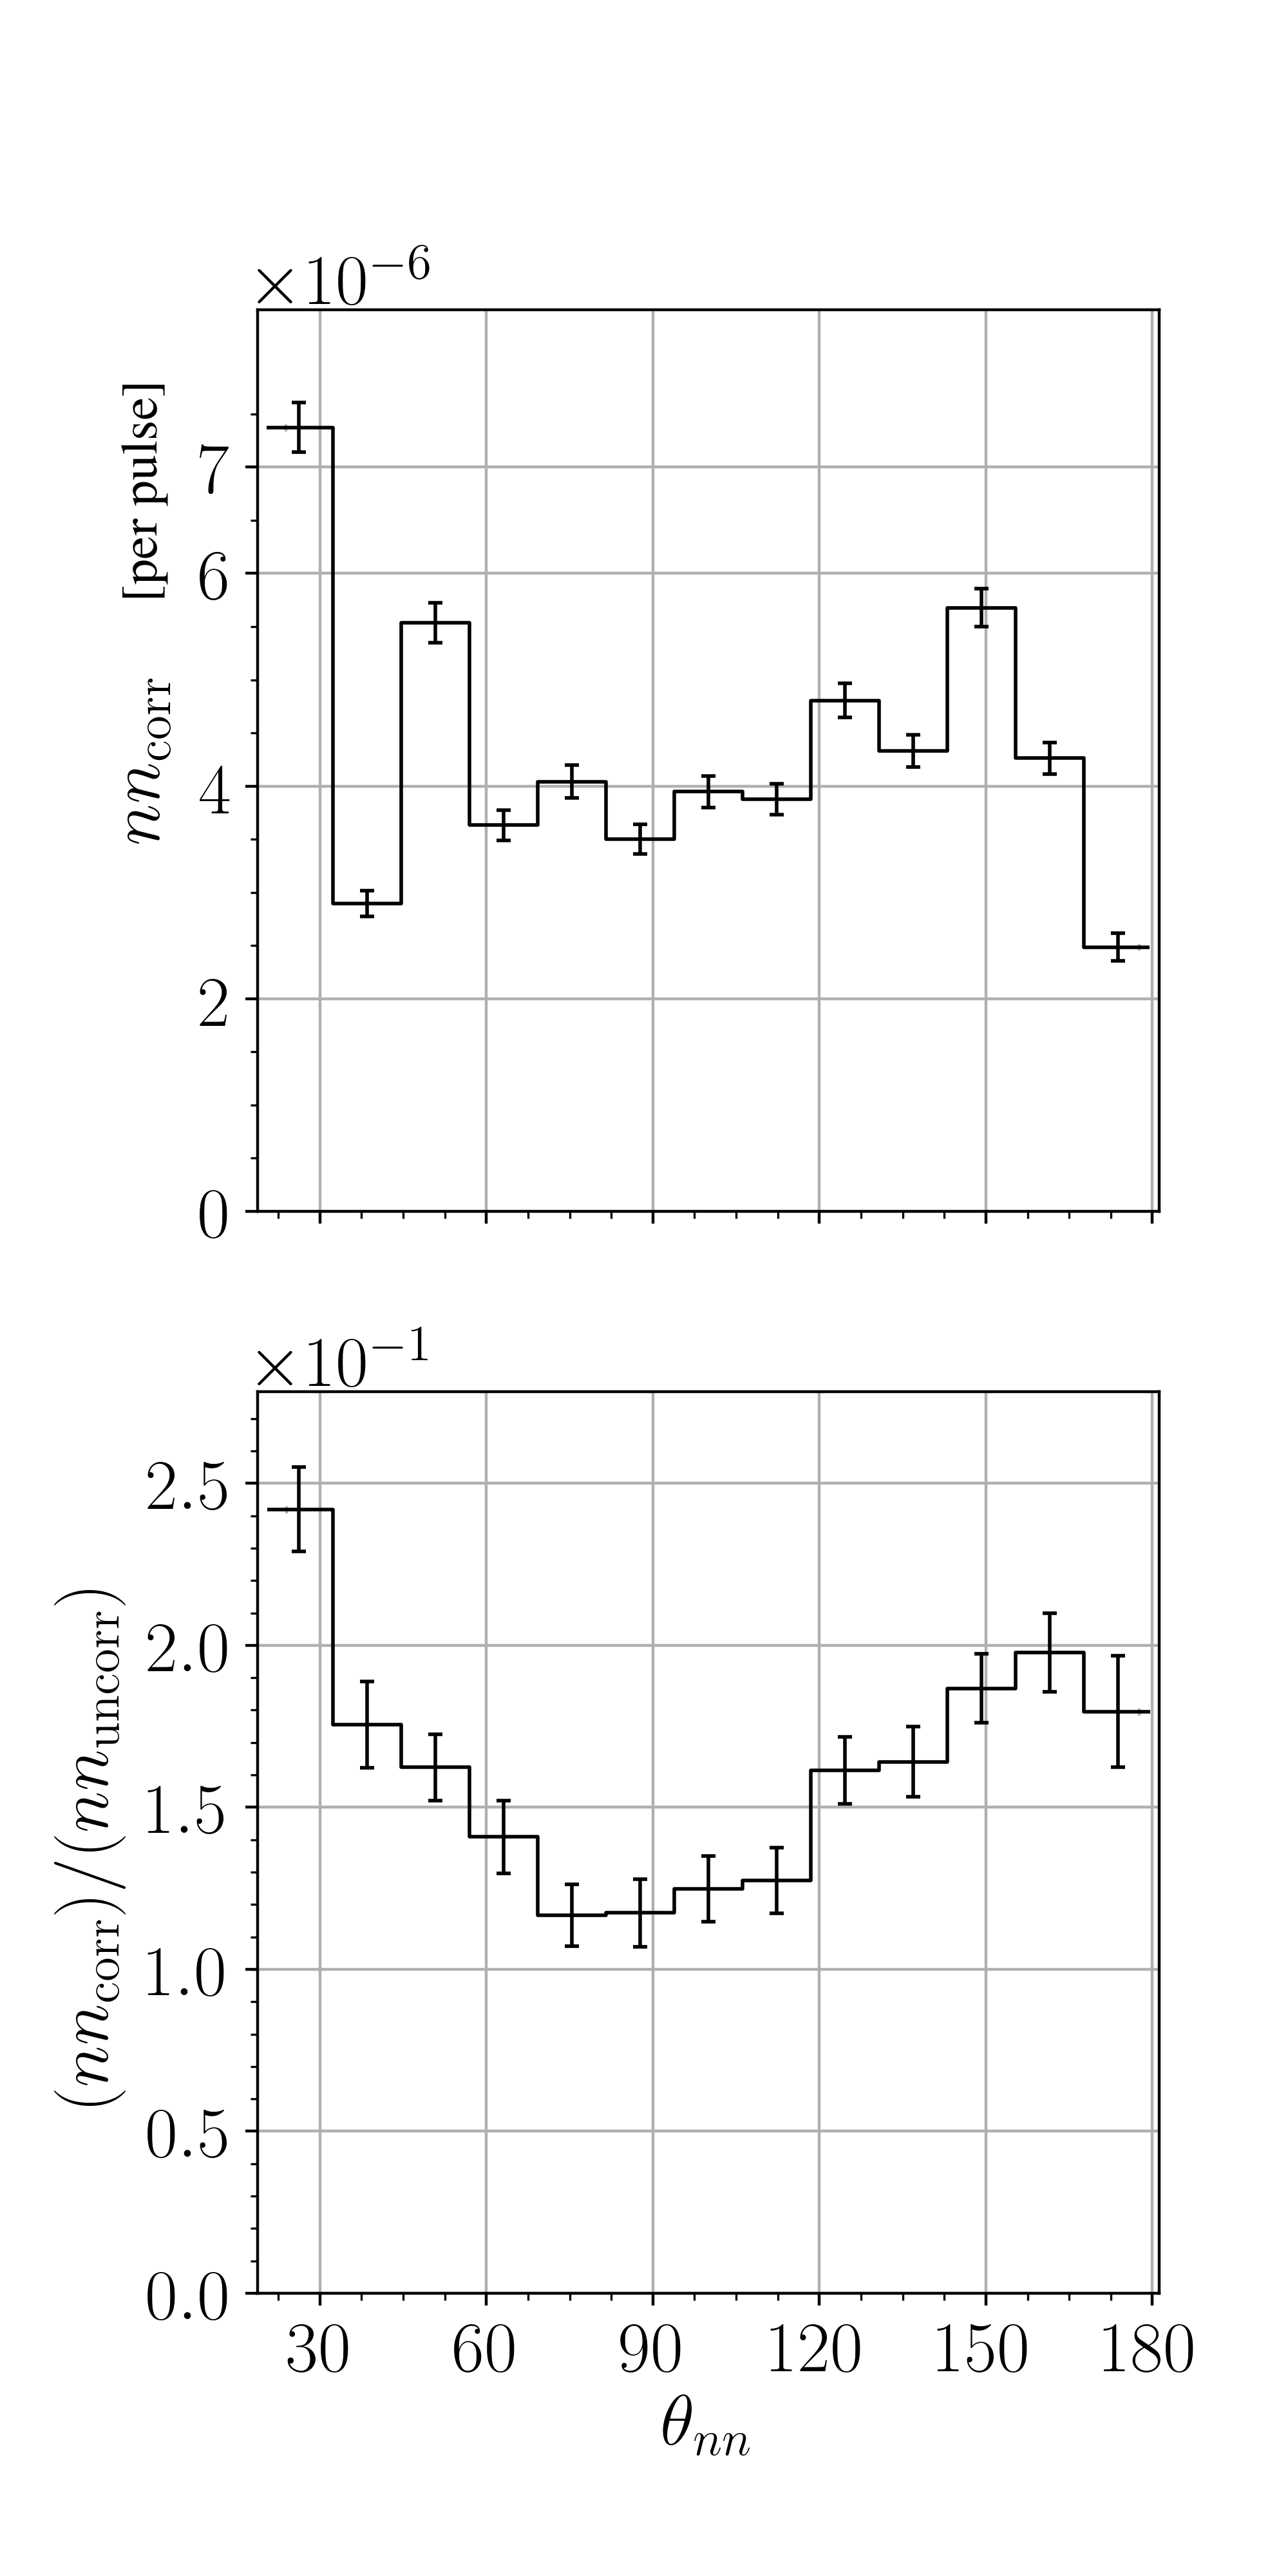
\includegraphics[width=\figsmall\textwidth]{SPDPNormalization.png}
    \caption{ n-n opening angle distribution from the photofission of $^{238}$U before the normalization procedure seen in Eq.~\ref{eq:angularCorr} (a), and after normalization (b).
    All measured neutrons have an energy greater than 0.4 MeV.}
    \label{fig:SPDPNormalization}
\end{figure}

\subsection{Subtraction of Accidental Coincidences}
\label{Reconstruction of Accidental Coincidence}
% explicity mention that nn_dp does not require each pulse to have two neutrons.  
The observation of two uncorrelated signals in the neutron ToF range, whether caused by neutrons, photons, or noise, is referred to as an \emph{accidental coincidence}.
%A small number of accidental coincidences are due to photons because the smeared gamma flash slightly overlaps with neutron ToF range.
Accidental coincidences due to noise and photons, which are estimated using a non-neutron producing aluminum target (see Fig.~\ref{fig:Noise}), amount to about 3\% of all coincidences.
Accidental coincidences due to neutrons are minimized by adjusting the accelerator's current so that there are, on average, less than 1.0 fissions per accelerator pulse.
Nevertheless, statistical fluctuations in the number of fissions per pulse result in the production of accidental coincident neutrons that originated from different, and therefore, uncorrelated fissions.
There are also accidental neutron coincidences caused by the occurrence of multiple $(\gamma, n)$ reactions in a single pulse.
The energy integrated $(\gamma, n)$ cross-section of $^{238}$U, weighted by the bremsstrahlung energy distribution, is about a factor of 5.5 times greater than it is for photofission (see Fig.~\ref{fig:CrossSection}).
As a result, the raw n-n coincident yield will contain a significant number of n-n coincidences from multiple $(\gamma, n)$ reactions in relation to n-n coincidences from fission.
The presence of accidental n-n coincidences has the effect of washing out the signal from correlated neutrons. 
\begin{figure}[]
\centering
    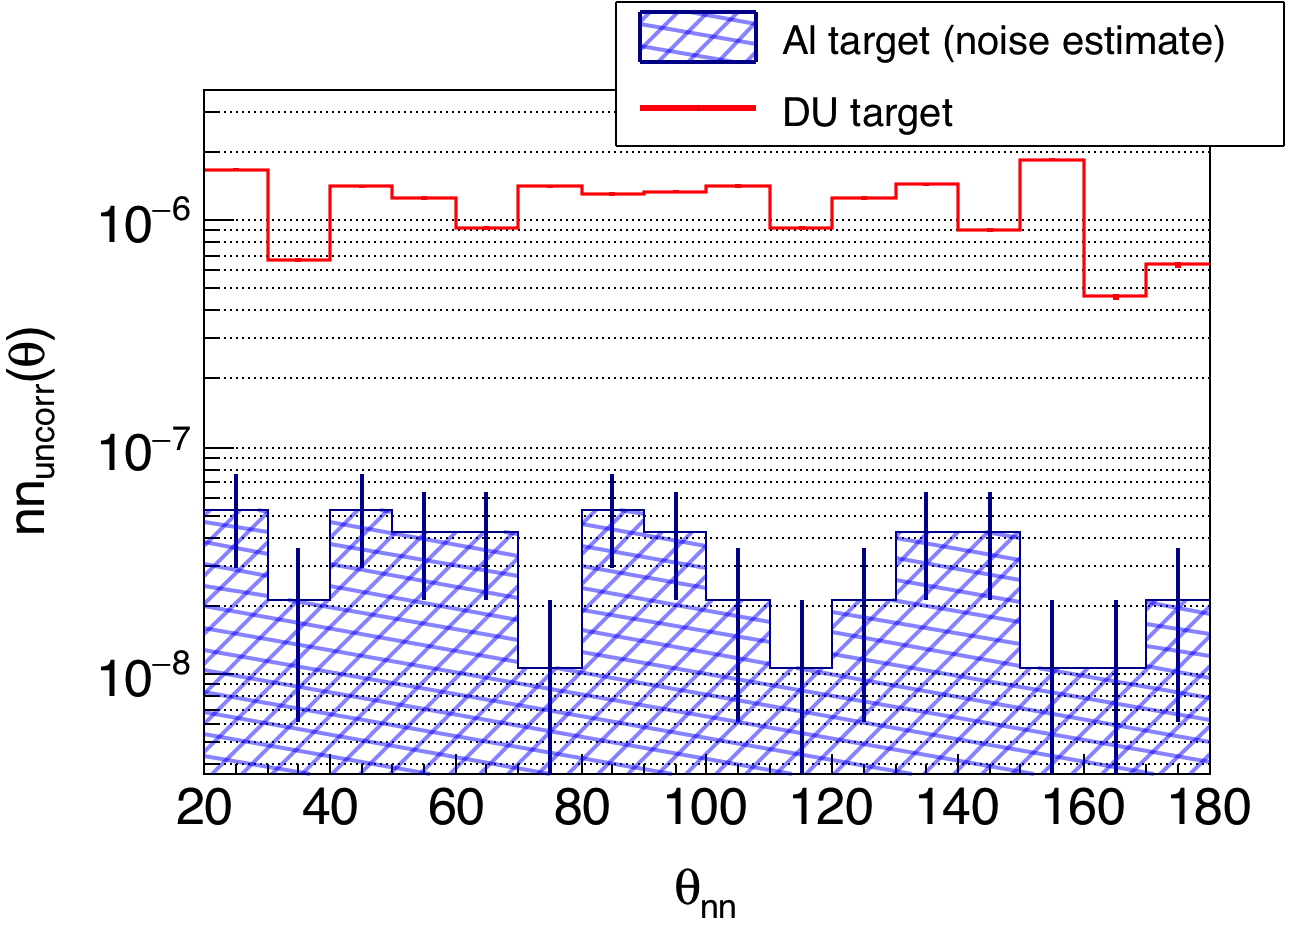
\includegraphics[width=\figsize\textwidth]{Noise.png}
    \caption{An Al target was designed have the same thickness, in radiation lengths, as the $^{238}$U target, thus serving as an equivalent non-neutron producing target well-suited for noise estimates.
    The rate of the detection of coincident events in the neutron ToF range while using the Al target was 3\% that of the $^{238}$U target.
    Thus, 3\% of coincident events used in the determination of n-n angular correlations in $^{238}$U can be attributed to noise.
        }
    \label{fig:Noise}
\end{figure}
\begin{figure}[]
\centering
    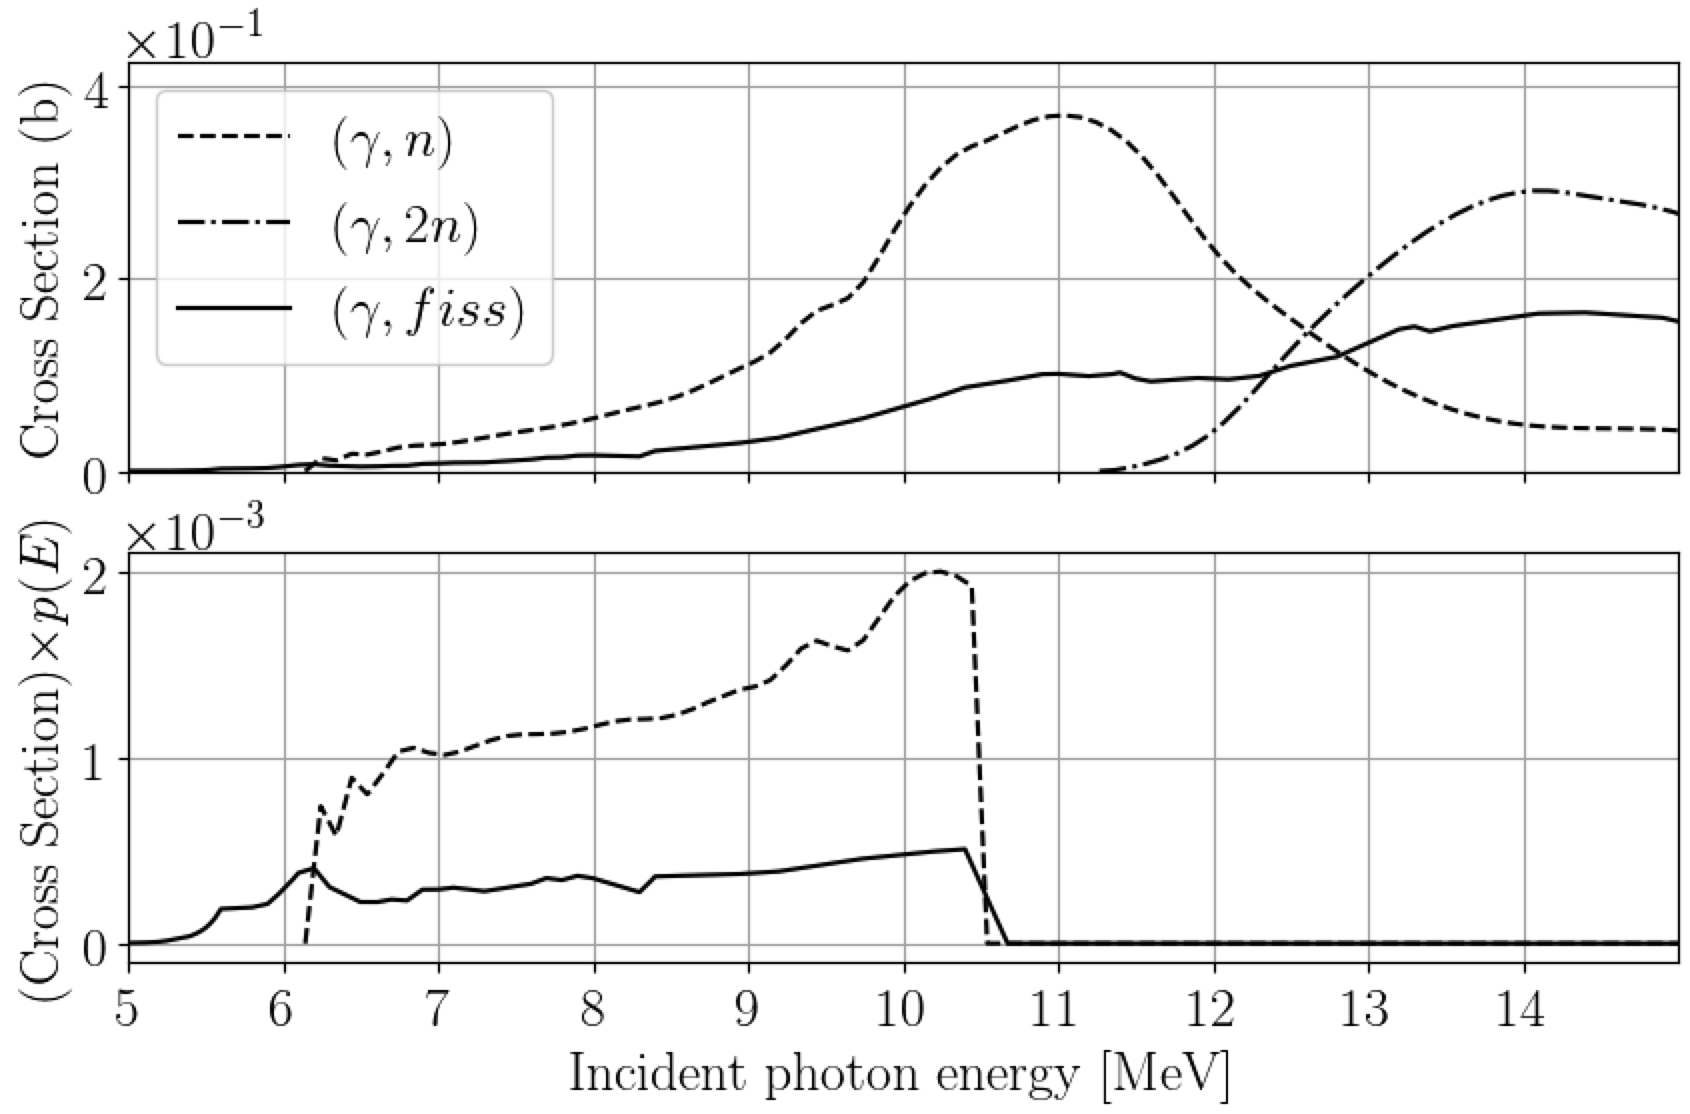
\includegraphics[width=\figsize\textwidth]{CrossSections.png}
    \caption{(top) ENDF cross-sections of $(\gamma$,fiss), direct $(\gamma$,n), and direct $(\gamma$,2n).
    (bottom) Cross-sections weighted by the simulated relative rate of bremsstrahlung photons that reach the target as a function of photon energy. 
    The integrated cross-sections of $(\gamma, n)$ is 5.5 times greater than for $(\gamma, \text{fiss})$. 
    Assuming a $\overline{\nu}$ of 2 neutrons/fission, the bremsstrahlung beam produces about 2.7 times more neutrons via $(\gamma$,n) than $(\gamma$,fiss) within the target.
        \label{fig:CrossSection}
        }
\end{figure}

The raw measurement of n-n yield consists of a mix of correlated and accidental neutron coincidences, that is
\begin{equation}
\label{eq:corr_uncorr}
nn_{\text{raw}}(\theta_{nn})= nn_{\text{corr}}(\theta_{nn}) + nn_{\text{acc}}(\theta_{nn}) \, ,
\end{equation}
where $nn_{\text{raw}}(\theta_{nn})$ and $nn_{\text{acc}}(\theta_{nn})$ are the per-pulse n-n yields as a function of opening angle, $\theta_{nn}$, for all detected n-n pairs, and detected accidental n-n pairs, respectively. As already defined, $ nn_{\text{corr}}(\theta_{nn})$ is the per-pulse yield of detected correlated n-n pairs.

Because the n-n coincidences comprising $nn_{\text{acc}}(\theta_{nn})$ consist of two independent detected neutrons, they are governed by the exact same physics and are subject to the exact same experimental conditions as n-n coincidences formed by pairing of single neutrons that were detected during different pulses.
% given that the two different pulses occurred at virtually the same time and thus under the same experimental conditions.
Therefore, the opening angle distribution formed by pairing neutrons that were detected during different pulses, denoted $nn_{dp}(\theta_{nn})$, is proportional to $nn_{\text{acc}}(\theta_{nn})$.
$nn_{dp}(\theta_{nn})$ is constructed from the set of all possible pulse-pairs formed by pulses that occurred within 0.2 seconds of each other.
The restriction in time difference is applied in order to increase the chance that pulse pairs together occurred under similar experimental conditions.
There are no other restrictions on which pulses can be used in this case.
Many pulse-pairs used for the construction of $nn_{dp}(\theta_{nn})$ will contain no detected neutrons.
% This is different than the construction of $nn_{\text{uncorr}}(\theta_{nn})$, which only used pulse-pairs in which there was an n-n coincidence in both pulses.

While $nn_{dp}(\theta_{nn})$ and $nn_{\text{acc}}(\theta_{nn})$ are proportional, $nn_{\text{acc}}(\theta_{nn})$ is not equal to $nn_{dp}(\theta_{nn})$,  because there are, on average, more detected neutrons per pulse-pair than per pulse.
As the following analysis shows,~$nn_{\text{acc}}(\theta_{nn}) = \frac{1}{2}nn_{dp}(\theta_{nn})$, under the condition that $nn_{\text{acc}}(\theta_{nn})$ is normalized to the number of pulses and $nn_{dp}(\theta_{nn})$ to the number of pulse-pairs looked at.
When looking at single pulses, the probability of there being a detected uncorrelated n-n pair is denoted by $P^{\text{n-n}}_{\text{sp}}$, and when looking at pulse-pairs, by $P^{\text{n-n}}_{\text{dp}}$.
Thus, $P^{\text{n-n}}_{\text{sp}}$ and $P^{\text{n-n}}_{\text{dp}}$ determine the relative rates of $nn_{\text{acc}}(\theta_{nn})$ and $nn_{dp}(\theta_{nn})$, respectively.

The statistics of the detected uncorrelated neutrons per pulse is assumed to follow a Poisson distribution, which describes the occurrence of independent random events.
Accordingly, the probability of the detection of $k$ uncorrelated neutrons in a given pulse is
\begin{equation} \label{math:Pois}
p(k) = \frac{e^{-\lambda}\lambda^{k}}{k!} \, ,
\end{equation}
where $\lambda$ represents the mean number of uncorrelated detected neutrons per pulse.
In principle, $\lambda$ equals the total number of detected uncorrelated neutrons divided by the total number of pulses.
%Data from the present experiment consists of accelerator pulses resulting in the detection of either zero, one, or two neutrons.
%All detected neutrons from accelerator pulses which yield one detected neutron are counted towards the total number of detected uncorrelated neutrons.
%Accelerator pulses which yield two detected neutrons, however, are counted in one of the following two ways: if the two detected neutrons are uncorrelated, then both neutrons are counted, and, if the two detected neutrons are correlated, then only one is counted because Poissonian statistics can only account for a strictly independent and uncorrelated set of random events.
%The resulting number of detected neutrons counted is then divided by the total number of pulses to give $\lambda$.
Determination of $\lambda$ cannot be done in practice, because one would need to know which pairs of detected neutrons are correlated.
However, the largest possible value for $\lambda$ is the total number of detected neutrons divided by the total number of pulses, as this quantity counts all detected neutrons, whether they are correlated or uncorrelated.
For this work, that places an upper bound on $\lambda$ of $5.5\times 10^{-3}$ detected uncorrelated neutrons per pulse, which is small enough to truncate all terms beyond the leading term in the following analysis.

%The probability of there being a detected uncorrelated n-n pair is denoted by $P^{\text{n-n}}_{\text{sp}}$ when looking at single pulses, and by $P^{\text{n-n}}_{\text{dp}}$ when looking at pulse-pairs.
%As explained above, the set of all detected uncorrelated n-n pairs from the same pulse (from which $nn_{\text{acc}}(\theta_{nn})$ is derived) and the set of all detected uncorrelated n-n pairs from different-pulse pairs (from which $nn_{dp}(\theta_{nn})$ is derived) are governed by the exact same physics and are subject to the exact same experimental conditions.
%The only difference between $nn_{dp}(\theta_{nn})$ and $nn_{\text{acc}}(\theta_{nn})$ is statistical, in that detected n-n pairs occur twice as frequently in $nn_{dp}(\theta_{nn})$ than in $nn_{\text{acc}}(\theta_{nn})$.
%Thus, all that remains to be shown is that  $P^{\text{n-n}}_{\text{sp}} = \frac{1}{2} P^{\text{n-n}}_{\text{dp}}$

Because $P^{\text{n-n}}_{\text{sp}}$ represents the probability of the detection of two uncorrelated neutrons in a single pulse, $P^{\text{n-n}}_{\text{sp}}$ is equal to $p(2)$, as per Eq.~\ref{math:Pois}.
Thus, 
%The accidental coincidence rate per pulse integrated over all opening angles, denoted by $\sum_{\theta_{nn}} nn_{\text{acc}}(\theta_{nn})$, is equal to the probability of there being exactly two detected uncorrelated neutrons detected in a single pulse
%\footnote{Cases of greater than two-fold coincidence are not considered in this analysis, as it is not necessary because of the low detection rates during this work.}:% It can be shown, however, that accounting for any number of coincidences, from zero all the way up to $\infty$-fold coincident events in a pulse or pulse-pair, will give the same answer.}:
\begin{equation} \label{math:SP}
    \begin{split}
    P^{\text{n-n}}_{\text{sp}} & = \frac{e^{-\lambda}\lambda^{2}}{2!} \\
        &\approx \frac{\lambda^2}{{2}} + \mathcal{O}(\lambda^3) \, .
    \end{split}
\end{equation}

When considering the case of $P^{\text{n-n}}_{\text{dp}}$, recall that, in this case, uncorrelated n-n pairs are formed by examining pulse-pairs.
Here, an uncorrelated n-n pair occurs when there is a detected neutron in both pulses.
Because all terms beyond the leading term are being truncated, pulse-pairs in which one or both of the pulses comprise two or more detected neutrons do not need to be considered.
Thus, $P^{\text{n-n}}_{\text{dp}}$ is equal to the probability of there being exactly one detected neutron in each pulse, which is the square of the probability of there being exactly one detected neutron in a single pulse, namely, $p(1)^2$. %in Eq.~\ref{math:SP}.
Thus, again using Eq.~\ref{math:Pois},
\begin{equation} \label{math:DP}
    \begin{split}
  P^{\text{n-n}}_{\text{dp}}&= \left(e^{-\lambda}\lambda\right)^{2} \\
    &\approx \lambda^2 + \mathcal{O}(\lambda^3) \, .
    \end{split}
\end{equation}

Because $P^{\text{n-n}}_{\text{dp}}$ and $P^{\text{n-n}}_{\text{sp}}$ determine the relative rates of $nn_{dp}(\theta_{nn})$ and $nn_{\text{acc}}(\theta_{nn})$, respectively, and because the two distributions have the same shape, from Eq.'s (\ref{math:DP}) and (\ref{math:SP}), it follows that
\begin{equation}
\label{eq:uncorr_DP}
nn_{\text{acc}}(\theta_{nn}) = \frac{1}{2}nn_{dp}(\theta_{nn}) \,.
\end{equation}
Finally, from Eq.'s ~\ref{eq:uncorr_DP} and~\ref{eq:corr_uncorr}, the distribution of solely correlated n-n pairs can be recovered from the raw measurement as follows
\begin{equation}
\label{math:acc_final}
nn_{\text{corr}}(\theta_{nn}) = nn_{\text{raw}}(\theta_{nn}) - \frac{1}{2}nn_{dp}(\theta_{nn}) \,.
\end{equation}
